\section{Модель нагрева слоя ПММА при экспонировании}

Выделение энергии в резисте при его экспонировании электронным лучом может приводить к нагреву резиста. Поскольку в методе СЭЛТР температура резиста непосредственным образом определяет интенсивность различных процессов, приводящих к формированию конечного профиля, необходимо оценить, насколько повышается температура ПММА в центре линии при экспонировании. Для этого в данной работе было использовано математическое моделирование.

Моделирование нагрева слоя ПММА проводилось на основе подхода, описанного в разделе~\ref{sec:sim_heating} для следующих условий экспонирования: ток экспонирования -- 5 нА, энергия электронного пучка -- 20 кэВ, размеры экспонируемой области -- 2.4$\times$1.9 мм$\pp$, толщина слоя ПММА -- 900 нм, число линий в кадре -- 625, расстояние между линиями -- 3 мкм, время экспонирования -- 100 с, температура образца -- 130~$^\circ$C. Для вычисления интегралов в формуле~\ref{eq:heat_final_equation} использовался метод Монте-Карло, что позволило достичь компромисса между машинным временем, необходимым для вычислений и точностью вычислений.

Результаты моделирования температуры ПММА при экспонировании показало, что увеличение температуры в центре линии составляет менее 1~$^\circ$C (рисунок~\ref{fig:heating}). Это позволило в дальнейшем считать, что при экспонировании ПММА ``в кадр'' при характерных размерах области экспонирования порядка нескольких миллиметров и токе экспонирования в диапазоне 1-10 нА повышением температуры ПММА можно пренебречь.

\begin{figure}[h!]
	\begin{center}
		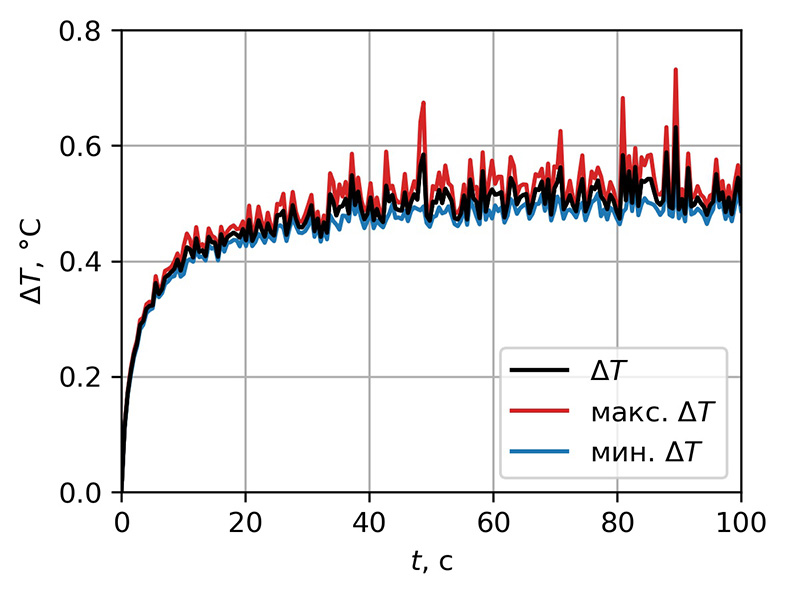
\includegraphics[width=0.6\linewidth]{heating/heating_200.jpg}
	\end{center}
	\vspace{-1em}
	\caption{Промоделированное увеличение температуры ПММА в центре линии при экспонировании ``в кадр''. Ток экспонирования -- 5 нА, энергия электронного пучка -- 20 кэВ, размеры экспонируемой области -- 2.4$\times$1.9 мм$\pp$, толщина слоя ПММА -- 900 нм, число линий в кадре -- 625, расстояние между линиями -- 3 мкм, время экспонирования -- 100 с, температура образца -- 130~$^\circ$C. Наличие минимального и максимального значений $\Delta T$ обусловлено использованием метода Монте-Карло для вычисления интегралов в формуле~\ref{eq:heat_final_equation}.}
	\label{fig:heating}
\end{figure}




